\documentclass[aspectradio=43]{beamer}
\usetheme{Berlin}
\usecolortheme{crane}

\usepackage[spanish]{babel}
\usepackage[utf8]{inputenc}
\usepackage{graphicx}
\usepackage{lipsum}
\usepackage{listings}
\usepackage{xcolor}
\usepackage{tabularx}
\usepackage{colortbl}

\title{Resumen de la arquitectura ARMv8}
\subtitle{Organización del Computador - Prácticos 6,7,8 y 9}
\author{Pedro Villar}
\date{\today}

\begin{document}
\begin{frame}
    \titlepage
\end{frame}

\section{Aritmética}
\begin{frame}
    \begin{table}
        \frametitle{Operaciones aritméticas - Suma y resta}
        \begin{tabular}{|c|c|c|}
            \hline
            \rowcolor{orange!20}
            \textbf{Intrucción} & \textbf{Sintaxis} & \textbf{Significado} \\
            \hline
            \texttt{ADD} & \texttt{ADD X0, X1, X2} & \texttt{X0 = X1 + X2} \\
            \texttt{SUB} & \texttt{SUB X0, X1, X2} & \texttt{X0 = X1 - X2} \\
            \texttt{ADDI} & \texttt{ADDI X0, X1, \#3} & \texttt{X0 = X1 + 3} \\
            \texttt{SUBI} & \texttt{SUBI X0, X1, \#3} & \texttt{X0 = X1 - 3} \\
            \hline
        \end{tabular}
    \end{table}
    En las instrucciones \texttt{ADDI} y \texttt{SUBI} el tercer operando es un valor inmediato, se representa con \texttt{\#}.
\end{frame}

\begin{frame}[containsverbatim]
    \frametitle{\#1 Ejemplo de suma y resta}
    Supongamos que las variables \texttt{a,b,c,d,e} están almacenadas en los registros \texttt{X0,X1,X2,X3,X4} respectivamente.\\
    \begin{verbatim}
        a = b + c;
        d = a - e;
    \end{verbatim}
    El código ensamblador sería:
    \begin{verbatim}
        ADD X0, X1, X2
        SUB X3, X0, X4
    \end{verbatim}
\end{frame}

\begin{frame}[containsverbatim]
    \frametitle{\#2 Ejemplo de suma y resta}
    Supongamos que las variables \texttt{f,g,h,i,j} están almacenadas en los registros \texttt{X0,X1,X2,X3,X4} respectivamente.\\
    \begin{verbatim}
        f = (g + h) - (i + j);
    \end{verbatim}
    El código ensamblador sería:
    \begin{verbatim}
        ADD X0, X1, X2 // X0 = g + h
        ADD X3, X3, X4 // X3 = i + j
        SUB X0, X0, X3 // X0 = (g + h) - (i + j)
    \end{verbatim}
\end{frame}

\section{Uso de memoria}
\begin{frame}
    \frametitle{Operandos de memoria}
    La memoria podría pensarse como un arreglo unidimensional grande, donde la dirección actúa como el índice del arreglo. LEGv8 utiliza direccionamiento por bytes, donde cada palabra representa 8 bytes.\\
    \begin{figure}
        \centering
        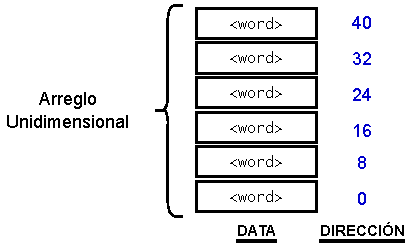
\includegraphics[width=0.5\textwidth]{static/memoria.pdf}
        \caption{Dirección de memoria}
    \end{figure}
\end{frame}

\begin{frame}
    \frametitle{Operandos de memoria - LDUR}
    La intrucción de transferencia de datos \texttt{LDUR} copia información desde la memoria hacia un registro que se denomina \textit{carga (LOAD)}. El formato de la instrucción consta de el registro en el que se cargará, seguido del registro junto con la constante usada para acceder a la memoria. Donde la suma de los valores del registro y la constante se usan para acceder a la memoria.\\
\end{frame}

\begin{frame}
    \frametitle{Acceso a direcciones de memoria}
    Como LEGv8 utiliza direccionamiento por bytes, cuando un array que se almacena en memoria continuamente quiere ser accedido, se debe tener en cuenta que la dirección de memoria se incrementa en 8 bytes por cada elemento del array. Por ejemplo, si se busca acceder al elemento 7 de un array, el desplazamiento que se le debe agregar al registro base del array es \(8 \times 7 = 56 \) y por lo tanto para guardar lo que esta en $A[7]$, suponiendo que la dirección base del array es \(X0\), la instrucción sería \texttt{LDUR X1, [X0, \#56]}.
\end{frame}

\begin{frame}[containsverbatim]
    \frametitle{Ejemplo de acceso a memoria - LDUR}
    Supongamos que la dirección base del array $A$ es \(X22\) y la variable $h$ esta almacenada en el registro \(X21\).\\
    \begin{verbatim}
        h = A[8];
    \end{verbatim}
    El código ensamblador sería:
    \begin{verbatim}
        LDUR X21, [X22, #64]
    \end{verbatim} 
\end{frame}

\begin{frame}
    \frametitle{Operandos de memoria - STUR}
    La instrucción complementaria a \textit{"load"} se denomina \textit{"store"}, esta instrucción copia datos desde un registro hacia la memoria. El formato de la instrucción es: el registro que se almacenará en memoria, seguido del registro base y la constante que se usará para el desplazamiento.\\
\end{frame}

\begin{frame}[containsverbatim]
    \frametitle{Ejemplo de acceso a memoria - STUR}
    Supongamos que la variable $h$ esta almacenada en el registro \(X21\) y la dirección base del array $A$ es \(X22\).\\
    \begin{verbatim}
        A[12] = h + A[8];
    \end{verbatim}
    El código ensamblador sería:
    \begin{verbatim}
        LDUR X23, [X22, #64] // X23 = A[8]
        ADD X21, X21, X23 // X21 = h + A[8]
        STUR X21, [X22, #96] // A[12] = h + A[8]
    \end{verbatim}
\end{frame}

\section{Operaciones lógicas}
\begin{frame}
    \frametitle{Operaciones lógicas}
    Las operaciones lógicas son instrucciones que se realizan bit a bit. Son utilizadas para examinar y modificar los bits de una palabra.
    \begin{table}
        \begin{tabular}{|c|c|c|}
            \hline
            \rowcolor{orange!20}
            \textbf{Operación Lógica} & \textbf{Instrucción} & \textbf{Sintaxis} \\
            \hline
            Shift Left & \texttt{LSL} & \texttt{LSL X0, X1, \#3} \\
            Shift Right & \texttt{LSR} & \texttt{LSR X0, X1, \#3} \\
            Bit-by-bit AND & \texttt{AND} & \texttt{AND X0, X1, X2} \\
            Bit-by-bit OR & \texttt{ORR} & \texttt{ORR X0, X1, X2} \\
            Bit-by-bit NOT & \texttt{EOR} & \texttt{EOR X0, X1, X2} \\
            \hline
        \end{tabular}
    \end{table}
\end{frame}

\begin{frame}
    \frametitle{Operaciones lógicas - Shift Left}
    La operación \texttt{LSL} realiza un desplazamiento a la izquierda de los bits de un registro. El número de bits que se desplazan se especifica en el tercer operando. Esta operación es equivalente a multiplicar por \(2^n\), donde \(n\) es el número de bits que se desplazan. \\
    Por ejemplo, si se desea multiplicar por 8 el contenido de \(X1\) y almacenarlo en \(X0\), la instrucción sería \texttt{LSL X0, X1, \#3}.
\end{frame}

\begin{frame}
    \frametitle{Operaciones lógicas - Shift Right}
    La operación \texttt{LSR} realiza un desplazamiento a la derecha de los bits de un registro. El número de bits que se desplazan se especifica en el tercer operando. Esta operación es equivalente a dividir por \(2^n\), donde \(n\) es el número de bits que se desplazan. \\
    Por ejemplo, si se desea dividir por 4 el contenido de \(X1\) y almacenarlo en \(X0\), la instrucción sería \texttt{LSR X0, X1, \#2}.
\end{frame}

\begin{frame}
    \frametitle{Operaciones Lógicas - AND}
    La operación \texttt{AND} realiza una operación bit a bit de la operación AND entre registros, basicamente toma bit a bit y realiza la operación AND, dejando un 1 si ambos bits son 1 y un 0 en caso contrario.\\
    Por ejemplo el registro \(X11\) contiene:
    \begin{equation*}
        \scriptstyle
        00000000\ 00000000\ 00000000\ 00000000\ 00000000\ 00000000\ 00001101\ 11000000
    \end{equation*}
    y el registro \(X10\) contiene:
    \begin{equation*}
        \scriptstyle
        00000000\ 00000000\ 00000000\ 00000000\ 00000000\ 00000000\ 00111100\ 00000000
    \end{equation*}
    La instrucción \texttt{AND X9, X10, X11} resultará en:
    \begin{equation*}
        \scriptstyle
        00000000\ 00000000\ 00000000\ 00000000\ 00000000\ 00000000\ 00001100\ 00000000
    \end{equation*}
\end{frame}

\begin{frame}
    \frametitle{Operaciones Lógicas - ORR}
    La operación \texttt{ORR} realiza una operación bit a bit de la operación OR entre registros, basicamente toma bit a bit y realiza la operación OR, dejando un 1 si al menos uno de los bits es 1 y un 0 en caso contrario.\\
    Por ejemplo el registro \(X11\) contiene:
    \begin{equation*}
        \scriptstyle
        00000000\ 00000000\ 00000000\ 00000000\ 00000000\ 00000000\ 00001101\ 11000000
    \end{equation*}
    y el registro \(X10\) contiene:
    \begin{equation*}
        \scriptstyle
        00000000\ 00000000\ 00000000\ 00000000\ 00000000\ 00000000\ 00111100\ 00000000
    \end{equation*}
    La instrucción \texttt{ORR X9, X10, X11} resultará en:
    \begin{equation*}
        \scriptstyle
        00000000\ 00000000\ 00000000\ 00000000\ 00000000\ 00000000\ 00111101\ 11000000
    \end{equation*}
\end{frame}

\begin{frame}
    \frametitle{Operaciones Lógicas - EOR y NOT}
    \begin{itemize}
        \item La operación \texttt{EOR} realiza una operación bit a bit de la operación XOR entre registros, basicamente toma bit a bit y realiza la operación XOR, dejando un 1 si los bits son diferentes y un 0 si son iguales.\\
        \item La operación \texttt{NOT} realiza una operación bit a bit de la operación NOT entre registros, basicamente toma bit a bit y realiza la operación NOT, dejando un 1 si el bit es 0 y un 0 si el bit es 1.
    \end{itemize}
\end{frame}

\section{Condicionales}
\begin{frame}
    \frametitle{Condicionales}
    El lenguaje ensamblador de LEGv8 posee dos instrucciones de este tipo, estas son \texttt{CBZ} y \texttt{CBNZ}.
    \begin{itemize}
        \item \texttt{CBZ registro, L1} Esta instrucción significa \textit{ir a la instrucción etiquetada L1 si el valor en el registro es igual a cero}. CBZ significa \textit{comparar y saltar si es cero}.
        \item \texttt{CBNZ registro, L1} Esta instrucción significa \textit{ir a la instrucción etiquetada L1 si el valor en el registro es diferente de cero}. CBNZ significa \textit{comparar y saltar si no es cero}.
    \end{itemize}
\end{frame}

\begin{frame}[containsverbatim]
    \frametitle{Ejemplo de condicionales}
    En el siguiente segmento de código, f, g, h, i y j son variables. Si las cinco variables f a j corresponden a los cinco registros X19 a X23, ¿cuál es el código LEGv8 compilado para esta instrucción if en C?\\
    \begin{verbatim}
        if (i == j) f = g + h; else f = g - h;
    \end{verbatim}
    La primera expresión compara la igualdad entre dos variables en registros. Dado que las instrucciones anteriores solo pueden probar si un registro es cero, el primer paso es restar j de i para probar si la diferencia es cero.
\end{frame}

\begin{frame}[containsverbatim]
    Parecería que luego querríamos ramificar si la diferencia es cero (CBZ). En general, el código será más eficiente si probamos la condición opuesta para saltar sobre el código que se ramifica si la diferencia no es igual a cero (CBNZ). De esta forma usariamos las dos instrucciones, usando el registro X9 para almacenar el resultado de restar j de i:
    \begin{verbatim}
    SUB X9,X22,X23  // X9 = i - j
    CBNZ X9, Else   // ir a Else si i != j (X9 != 0)
    \end{verbatim}
\end{frame}

\begin{frame}[containsverbatim] 
    Luego, si i es igual a j, queremos calcular f = g + h, y saltar sobre el cálculo de f = g - h. Por lo tanto, el código sería:
    \begin{verbatim}
    ADD X19, X20, X21 // f = g + h
    B Exit // saltar sobre Else, ir a Exit
    Else: SUB X19, X20, X21 // f = g - h
    Exit:
    \end{verbatim}
\end{frame}

\begin{frame}[containsverbatim]
    El código completo sería:
    \begin{verbatim}
    SUB X9,X22,X23  // X9 = i - j
    CBNZ X9, Else   // ir a Else si i != j (X9 != 0)
    ADD X19, X20, X21 // f = g + h
    B Exit // saltar sobre Else, ir a Exit
    Else: SUB X19, X20, X21 // f = g - h
    Exit:
    \end{verbatim}
    En pocas palabras, el código compara i y j, y si son iguales, calcula f = g + h; de lo contrario, calcula f = g - h.
\end{frame}

\begin{frame}[containsverbatim]
    \frametitle{Condicionales para bucles}
    Se asume que i y k se corresponden con los registros X22 y X24, y la base del arreglo save está en X25. ¿Cuál es el código ensamblador LEGv8 correspondiente a este código C?
    \begin{verbatim}
        while (save[i] == k) i += 1;
    \end{verbatim}
\end{frame}

\begin{frame}[containsverbatim]
    El primer paso es cargar \texttt{save[i]} en un registro temporal. Antes de poder cargar \texttt{save[i]} en un registro temporal, necesitamos su dirección. Antes de poder sumar i a la base del arreglo save para formar la dirección, debemos multiplicar el índice i por 8. Podemos usar un desplazamiento a la izquierda (LSL), ya que desplazar a la izquierda por 3 bits multiplica por $2^3$. Necesitamos agregarle la etiqueta Loop para poder regresar a esa instrucción al final del ciclo:
    \begin{verbatim}
    Loop: LSL X10,X22,#3  // X10 = i * 8
          ADD X10,X10,X25  // X10 = &save[i]
    \end{verbatim}
    Ahora podemos usar esa dirección para cargar save[i] en un registro temporal:
    \begin{verbatim}
        LDUR X9,[X10,#0]  // X9 = save[i]
    \end{verbatim}
\end{frame}

\begin{frame}[containsverbatim]
    La siguiente instrucción resta k de save[i] y coloca la diferencia en X11 para configurar la prueba del ciclo. Si X11 no es 0, entonces son desiguales \texttt{(save[i] != k)}:
    \begin{verbatim}
        SUB X11,X9,X24  // X11 = save[i] - k
    \end{verbatim}
    La siguiente instrucción realiza la prueba del ciclo, saliendo si \texttt{save[i] != k}:
    \begin{verbatim}
        CBNZ X11,Exit  // salir si save[i] != k
    \end{verbatim}
    Luego se suma 1 a i y se repite el ciclo:
    \begin{verbatim}
        ADD X22,X22,#1  // i += 1
        B Loop  // repetir el ciclo
        Exit:
    \end{verbatim}
\end{frame}

\begin{frame}[containsverbatim]
    El código completo sería:
    \begin{verbatim}
    Loop: LSL X10,X22,#3  // X10 = i * 8
          ADD X10,X10,X25  // X10 = &save[i]
          LDUR X9,[X10,#0]  // X9 = save[i]
          SUB X11,X9,X24  // X11 = save[i] - k
          CBNZ X11,Exit  // salir si save[i] != k
          ADD X22,X22,#1  // i += 1
          B Loop  // repetir el ciclo
    Exit:
    \end{verbatim}
\end{frame}

\section{Ejercicios}
\begin{frame}
    \frametitle{Ejercicio 7 - Práctico 6}
    \begin{figure}
        \centering
        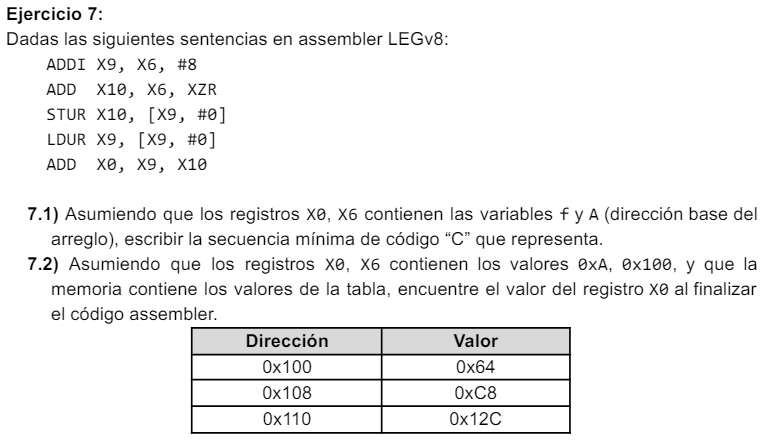
\includegraphics[width=0.8\textwidth]{static/ej7.png}
        \caption{Ejercicio 7 - Práctico 6}
    \end{figure}
\end{frame}

\begin{frame}[containsverbatim]
    Interpretación de las instrucciones:
    \begin{verbatim}
        ADDI X9, X6, #8 // X9 = &A[0] + 8 = A[1]
        ADD X10, X6, XZR // X10 = &A[0]
        STUR X10, [X9, #0] // A[1] = &A[0]
        LDUR X9, [X9, #0] // X9 = A[1]
        ADD X0, X9, X10 // f = A[0] + A[0]
    \end{verbatim}
    La secuencia mínima de C es:
    \begin{verbatim}
        f = A[0] + A[0];
    \end{verbatim}
    La dirección de memoria de A[0] es \(0x100\) y el contenido de A[0] es \(0x64\), entonces el programa definirá a X0 como \(0xC8\).
\end{frame}

\begin{frame}[containsverbatim]
    \frametitle{Ejercicio 8.1 - Práctico 6}
    Dado el contenido de los siguientes registros:
    \begin{itemize}
        \item[\textbf{a)}] X9 = 0x55555555, y X10=0x12345678
    \end{itemize}
    ¿Cuál es el valor del registro X11 luego de la ejecución del siguiente código
    assembler en LEGv8?
    \begin{verbatim}
        LSL X11, X9, #4
        ORR X11, X11, X10
    \end{verbatim}
\end{frame}

\begin{frame}
    El contenido de X9 puede ser representado como:
    \begin{equation*}
        \scriptstyle
        0101\ 0101\ 0101\ 0101\ 0101\ 0101\ 0101\ 0101
    \end{equation*}
    Despues de hacerle un desplazamiento a la izquierda de 4 bits, el contenido de X11 sería:
    \begin{equation*}
        \scriptstyle
        0101\ 0101\ 0101\ 0101\ 0101\ 0101\ 0101\ 0000
    \end{equation*}
    El contenido de X10 puede ser representado como:
    \begin{equation*}
        \scriptstyle
        0001\ 0010\ 0011\ 0100\ 0101\ 0110\ 0111\ 1000
    \end{equation*}    
    Por lo tanto, el contenido de X11 sería:
    \begin{equation*}
        \scriptstyle
        0101\ 0111\ 0111\ 0101\ 0101\ 0111\ 0111\ 1000 
    \end{equation*}
\end{frame}

\begin{frame}[containsverbatim]
    \frametitle{Ejercicio 1 - Práctico 7}
    Para estos dos programas con entrada y salida en X0, decir que función realizan:
    \begin{verbatim}
            SUBIS X0, X0, #0
            B.LT else
            B done
    else: SUB X0, XZR, X0
    done:
    \end{verbatim}
    \textbf{Respuesta:} El programa calcula el valor absoluto de X0.
\end{frame}

\begin{frame}[containsverbatim]
    \begin{verbatim}
          MOV X9, X0
          MOV X0, XZR
    loop: ADD X0, X0, X9
          SUBI X9, X9, #1
          CBNZ X9, loop
    done:
  \end{verbatim}
    \textbf{Respuesta:} El programa calcula el valor de la suma de los números de 0 a X0.
\end{frame}

\begin{frame}
    \frametitle{MOVZ y MOVK}
    Las instrucciones \texttt{MOVZ} y \texttt{MOVK} son instrucciones de carga inmediata. La instrucción \texttt{MOVZ} carga un valor inmediato en un registro dejando los demas bits en cero, mientras que la instrucción \texttt{MOVK} carga un valor inmediato en un registro, pero solo en los bits especificados por la máscara.\\
    \begin{table}
        \begin{tabular}{|c|c|c|}
            \hline
            \rowcolor{orange!20}
            \textbf{Instrucción} & \textbf{Sintaxis} & \textbf{Significado} \\
            \hline
            \texttt{MOVZ} & \texttt{MOVZ X0, \#0x1234, LSL \#0} & \texttt{X0 = 0x1234} \\
            \texttt{MOVK} & \texttt{MOVK X0, \#0x5678, LSL \#16} & \texttt{X0 = 0x12345678} \\
            \hline
        \end{tabular}
    \end{table}
\end{frame}

\section{Comparaciones}
\begin{frame}
    \frametitle{Comparaciones}
    El conjunto completo de comparaciones para números incluye menor que ($<$), menor o igual que ($\leq$), mayor que ($>$), mayor o igual que ($\geq$), igual ($=$) y diferente ($\neq$). La comparación de patrones de bits también debe considerar la diferencia entre números con signo y sin signo. En los números con signo, un patrón de bits con un 1 en el bit más significativo representa un número negativo y, por supuesto, es menor que cualquier número positivo, que debe tener un 0 en el bit más significativo.
\end{frame}

\begin{frame}
    \frametitle{FLAGS}
    En LEGv8, existen cuatro bits de condición, que registran el resultado de una instrucción, llamados FLAGS:
    \begin{itemize}
        \item \textbf{Negativo (N):} el resultado que estableció el código de condición tenía un 1 en el bit más significativo (indicando un número negativo).
        \item \textbf{Cero (Z):} el resultado que estableció el código de condición fue 0.
        \item \textbf{Overflow (V):} el resultado que estableció el código de condición causó un overflow (el resultado era demasiado grande para ser representado).
        \item \textbf{Carry (C):} el resultado que estableció el código de condición produjo un carry del bit más significativo o un borrow en el bit más significativo.
    \end{itemize}
\end{frame}

\begin{frame}
    \frametitle{Salto condicional}
    Las instrucciones de salto condicional utilizan combinaciones de estos códigos de condición para realizar las comparaciones deseadas y los saltos. En la arquitectura LEGv8, esta instrucción de salto condicional se llama B.cond. La parte cond de la instrucción se puede usar con cualquiera de las instrucciones de comparación con signo:
\end{frame}

\begin{frame}
    \begin{table}
        \begin{tabular}{|c|c|c|}
            \hline
            \rowcolor{orange!20}
            \textbf{Instrucción} & \textbf{Sintaxis} & \textbf{Significado} \\
            \hline
            \texttt{B.EQ} & \texttt{B.EQ L1} & \texttt{ir a L1 si Z = 1} \\
            \texttt{B.NE} & \texttt{B.NE L1} & \texttt{ir a L1 si Z = 0} \\
            \texttt{B.GE} & \texttt{B.GE L1} & \texttt{ir a L1 si N = V} \\
            \texttt{B.LT} & \texttt{B.LT L1} & \texttt{ir a L1 si N $\neq$ V} \\
            \texttt{B.GT} & \texttt{B.GT L1} & \texttt{ir a L1 si Z = 0 y N = V} \\
            \texttt{B.LE} & \texttt{B.LE L1} & \texttt{ir a L1 si Z = 1 o N $\neq$ V} \\
            \hline
        \end{tabular}
    \end{table}
\end{frame}

\begin{frame}[containsverbatim]
    \frametitle{Ejercicio 2 - Práctico 7}
    Dado el siguiente programa LEGv8, dar el valor final de X10, dado que inicialmente {X10=0x0000000000000001}.
    \begin{verbatim}
          SUBIS XZR, X9, #0
          B.GE else
          B done
    else: ORRI X10, XZR, #2
    done:
    \end{verbatim}
    \textbf{1.1:} Dado que inicialmente {X9=0x0000000000101000}.
\end{frame}

\begin{frame}
    \textbf{1.1:} Dado que inicialmente {X9=0x0000000000101000}.
    \begin{itemize}
        \item \texttt{SUBIS XZR, X9, \#0} \textit{XZR = 0x0000000000000000}
        \item \texttt{B.GE else} \textit{No se cumple la condición, se salta a la siguiente instrucción}
        \item \texttt{ORRI X10, XZR, \#2} \textit{X10 = 0x0000000000000002}
        \item \texttt{done:} \textit{Fin del programa}
        \item \textbf{Resultado:} \textit{X10 = 0x000 0000 0000 0002}
    \end{itemize}
    El programa asigna el valor 2 a X10.
\end{frame}

\end{document}